\documentclass[tikz,border=5mm]{standalone}
\usepackage{tikz}
\usetikzlibrary{arrows.meta,positioning,shapes.geometric}

\begin{document}
    % TikZの描画環境
    % node distanceでノード間のデフォルト距離を設定
    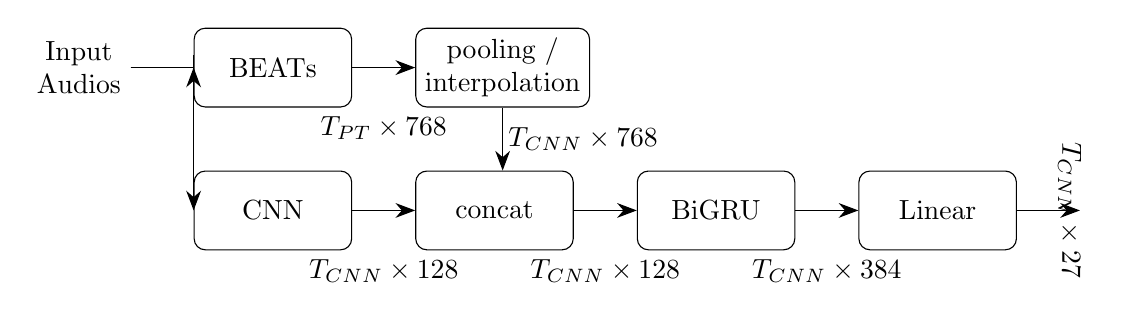
\begin{tikzpicture}[
        node distance=0.8cm and 0.8cm,
        % 各要素のスタイルを定義
        block/.style={
            rectangle, 
            rounded corners, 
            draw, 
            minimum width=2cm, 
            minimum height=1cm, 
            align=center
        },
        io/.style={
            align=center
        },
        % 矢印のスタイルを定義
        line/.style={
            draw, 
            -{Stealth[length=2.5mm]} % 矢印の先端の形と大きさ
        }
    ]

    % --- ノードの配置 ---
    % 座標(0,0)に最初のノードを配置
    \node[io] (input) {Input \\ Audios};

    % "input"ノードの右側に"pre"ノードを配置
    \node[block, right=of input] (pre) {BEATs};
    
    % "pre"ノードの下側に"cnn"ノードを配置
    \node[block, below=of pre] (cnn) {CNN};

    % "pre"ノードの右側に"pool"ノードを配置
    \node[block, right=of pre] (pool) {pooling / \\ interpolation};

    % "cnn"ノードの右側に"concat"ノードを配置
    \node[block, right=of cnn] (concat) {concat};

    % "concat"ノードの右側に"bigru"ノードを配置
    \node[block, right=of concat] (bigru) {BiGRU};

    % "bigru"ノードの右側に"linear"ノードを配置
    \node[block, right=of bigru] (linear) {Linear};

    % "linear"ノードの右側に"output"ノードを配置（枠なし）
    \node[right=of linear] (output) {}; % 矢印の終点


    % --- 矢印とラベルの描画 ---
    % |- を使うと、水平→垂直の線が引ける
    \path[line] (input.east) -| (pre.west);
    \path[line] (input.east) -| (cnn.west);

    % "pre"から"pool"への矢印と、その下のラベル
    \path[line] (pre.east) -- (pool.west) node[midway, below, yshift=-5mm] {$T_{PT} \times 768$};

    % "cnn"から"concat"への矢印と、その下のラベル
    \path[line] (cnn.east) -- (concat.west) node[midway, below, yshift=-5mm] {$T_{CNN} \times 128$};
    
    % "pool"から"concat"への矢印と、その上のラベル
    \path[line] (pool.south) -- (pool.south |- concat.north) node[midway, right, xshift=-0.5mm] {$T_{CNN} \times 768$};

    % "concat"から"bigru"への矢印と、その下のラベル
    \path[line] (concat.east) -- (bigru.west) node[midway, below, yshift=-5mm] {$T_{CNN} \times 128$};

    % "bigru"から"linear"への矢印と、その下のラベル
    \path[line] (bigru.east) -- (linear.west) node[midway, below, yshift=-5mm] {$T_{CNN} \times 384$};

    % "linear"から"output"への矢印と、その上のラベル
    \path[line] (linear.east) -- (output.west) node[midway, above, rotate=270] {$T_{CNN} \times 27$};

    \end{tikzpicture}
\end{document}
